% !TeX root = main.tex

\section{Theory: Non-holonomic Trajectory Planning using Bernstein Basis}

\label{sec:theory-nhtraj-bernstein}

This section only contains the theoretical background and procedure explanation for the assignment. It does not answer any specific question.

Proceed to section \ref{sec:note-custom-impl} for beginning of assignment submission.

\subsection{Bernstein Polynomials}

We generally use Bernstein Polynomials to approximate functions. They can also be used to generate trajectories through waypoints under certain constraints (as we will see here). This subsection explores only the polynomials.

A Bernstein polynomial is a linear combination of Bernstein basis polynomials \footnotemark[1]. The $n+1$ Bernstein basis polynomials of degree $n$ are given by the following equation.

\begin{equation}
    b_{v,n}(x) = \binom{n}{v} \; x^v \; (1-x)^{n-v}, \quad v = 0,\dots,n
    \label{eq:bernstein-basis-term}
\end{equation}

\subsection{Approximating functions}

For a continuous function $f$ defined in the interval $[0, 1]$, the following bernstein polynomial can be considered as a viable approximation.

\begin{equation}
    B_{n}(f)\,(x) = \sum_{v=0}^{n} f \left ( \frac{v}{n} \right ) b_{v, n} (x)
    \label{eq:bernstein-approx-func}
\end{equation}

The above approximation is more accurate if $n\rightarrow \infty$, that is $\underset{n \rightarrow \infty}{\textup{lim}} B_n(f) = f$.

Such a combination can be run through the waypoints (which will be presented as $f(\sfrac{v}{n})$ to the polynomial) to approximate the function to which those waypoints belong. An application of this method is to generate smooth splines through a given set of control points (called \emph{knots}) which is very useful in computer vision \footnotemark[2]. 

The basis function values for $n=5$ (fifth-degree) is shown in figure 

\begin{figure}[ht]
    \centering
    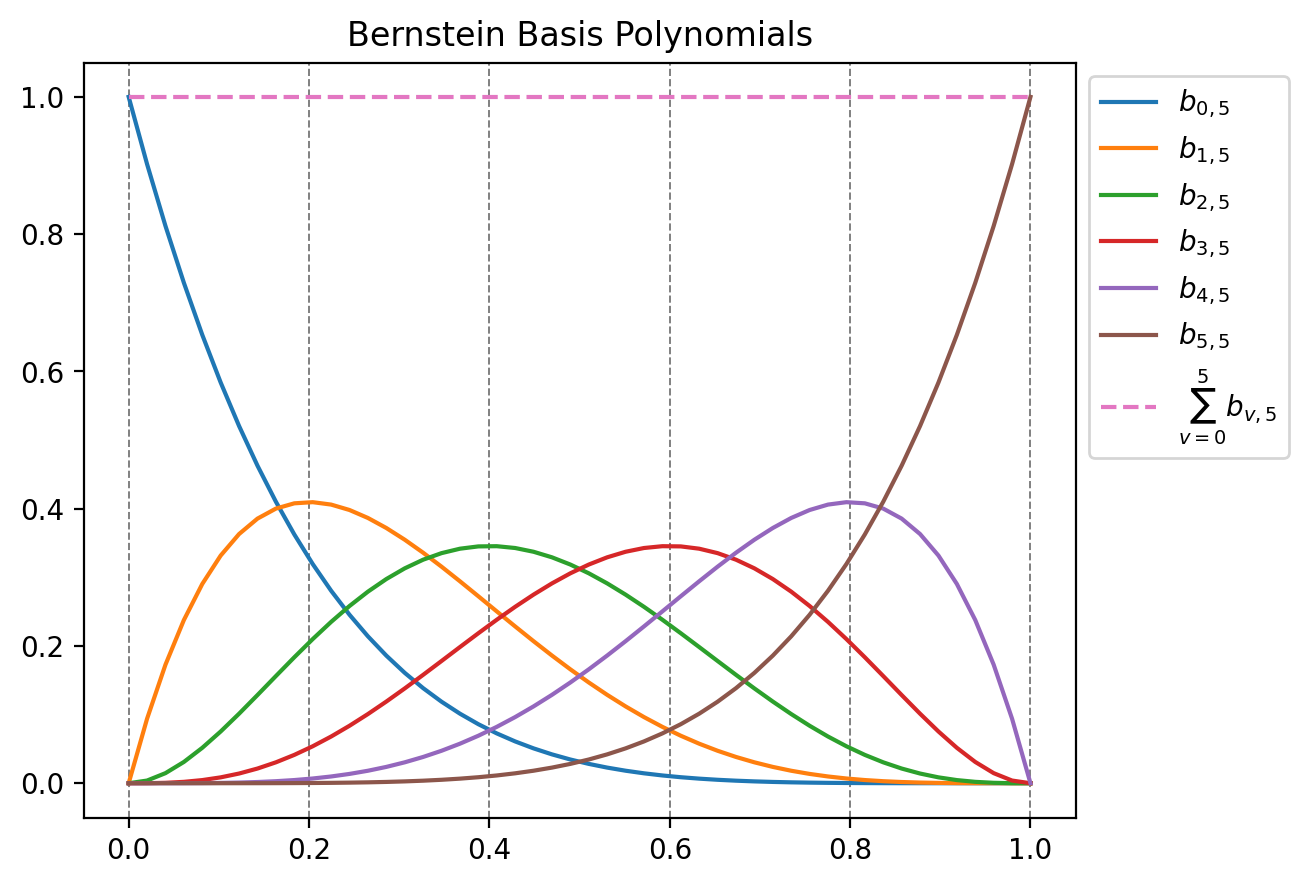
\includegraphics[width=0.5\textwidth]{bernstein_basis_values.png}
    \caption{Bernstein Basis Values for $n=5$}
    \label{fig:bernstein-basis-plots}
    \small
        Fifth order bernstein basis values. Note how for different $x = \sfrac{v}{n}$ (where $v = 0,\dots,n$), the corresponding $b_{v,n}(x)$ peaks, which shows the weight of the control point being considered. Here, the $b_{v,n}(x)$ values are weights and the $f\left(\sfrac{v}{n}\right)$ could be theorized as control points (the above graph only has $b$).

        This figure can be generated by running the \texttt{src/bernstein\_basis.py} script as main.

        \textbf{Note}: The sum of all bernstein basis polynomials at any instance $x$ is 1.
\end{figure}

\subsection{Non-Holonomic Path using Bernstein Polynomials}

In a non-holonomic system, the system loses its ability to freely move in space due to some physical limitations. A differential drive robot (or a car) cannot move sideways, its non-holonomic constrain stems from the way velocity is resolved along its center, that is

\begin{equation}
    \dot{x} = v \cos(\theta) \quad 
    \dot{y} = v \sin(\theta) \quad\quad
    \Rightarrow \dot{y} = \dot{x} \tan(\theta) \quad
    \Rightarrow y = \int{\dot{x} \tan \left ( \theta \right ) dt}
    \label{eq:diffdrive-non-holo-constraint}
\end{equation}

The above integral cannot be computed directly, only numerical solutions to it exits. The kinematic model of a differential drive robot is given by

\begin{align*}
    \dot{q} = \begin{bmatrix}
        \dot{x} \\ \dot{y} \\ \dot{\theta}
    \end{bmatrix} = \begin{bmatrix}
    \cos(\theta) & 0 \\
    \sin(\theta) & 0 \\
    0 & 1
    \end{bmatrix} \begin{bmatrix}
    v \\ \omega
    \end{bmatrix}
\end{align*}

In the above equations, the point  $x, y, \theta$ is the robot position (in the 2D planar environment) and $v, \omega$ are the velocity commands given to the robot body.

Since the system above loses a degree of freedom - it cannot move in all possible directions in the neighborhood, in other words it is \emph{not} holonomic - only two of $x, y, \theta$ can be independently modeled. 

\subsubsection{Problem Statement}

We are usually given the $x, y, \theta$ values at three points in time - the beginning $t_o$, waypoint $t_w$ or $t_c$, and end $t_f$. We are also given the first derivatives of $x$ at the time steps $t_o$, $t_c$, and $t_f$. We are also given $\dot{\theta}$ at time steps $t_o$ and $t_f$.

If this were holonomic (which it isn't), we could independently model the $x$, $y$, and $\theta$ as Bernstein polynomials and follow the given trajectory. But here, we have to use the constraint given by equation \ref{eq:diffdrive-non-holo-constraint}.

\subsubsection{Modeling \texorpdfstring{$x$ and $\tan(\theta)$}{x and tan}}

We model $x$ and $\tan(\theta)$ as degree $n=5$ Bernstein polynomials. Specifically, we do the following for $x$

\begin{equation}
    x(t) \approx B_n(x)(t) = B_n(x)(\mu(t)) = B_x(\mu(t)) = \sum_{i = 0}^{5} W_{x_i} B_i (\mu(t))
    \label{eq:x-bernstein-model}
\end{equation}

Note that the $x$ in the equations \ref{eq:bernstein-basis-term} and \ref{eq:bernstein-approx-func} mean an \emph{input} to some function (in the context of those equations). The $x$ in the above equation \ref{eq:x-bernstein-model} is \emph{itself a function} (not an input, the input here is time $t$).

The function $\mu(t) = \frac{t-t_o}{t_f - t_o} = \mu_t$ normalizes $t$ to be in the range $[0, 1]$. The Bernstein basis term therefore becomes $B_i(\mu(t)) = b_{i, 5}(\mu_t)$ (see equation \ref{eq:bernstein-basis-term} for expansion).

Also note that $W_{x_i}$ is a proxy for $x$ which decides the weight for a particular Bernstein basis $B_i$ (see figure \ref{fig:bernstein-basis-plots} for the plots).

The following can be done similarly for $\tan(\theta)$

\begin{equation}
    \tan \left( \theta(t) \right) = k(t) \approx B_k(\mu(t)) = \sum_{i = 0}^{5} W_{k_i} B_i (\mu(t))
    \label{eq:tan-bernstein-model}
\end{equation}

\subsubsection{Finding \texorpdfstring{$W_{x_i}$}{weights for x}}

We model the variable $x$ using equation \ref{eq:x-bernstein-model}.

\begin{equation}
    x(t) \approx B_n(x)(t) = \sum_{i = 0}^{5} W_{x_i} B_i (\mu(t))
    \tag{Eq. \ref{eq:x-bernstein-model} revisited}
\end{equation}

We model $\dot{x}$ as

\begin{equation}
    \dot{x}(t) = \sum_{i = 0}^{5} W_{x_i} \dot{B_i} (\mu(t))
    \label{eq:xdot-bernstein-model}
\end{equation}

We need to find the values for the $W_{x_i}$ terms (which are constants - they're weights of the Bernstein terms). We're given the values for $t_o$ (starting time), $t_w$ (waypoint time), $t_f$ (final time), $x(t_o) = x_o$, $x(t_w) = x_w$, $x(t_f) = x_f$ ($x$ at start, waypoint, and end time), $\dot{x}(t_o) = \dot{x}_o$, $\dot{x}(t_w) = \dot{x}_w$, and $\dot{x}(t_f) = \dot{x}_f$ ($\dot{x}$ at start, waypoint, and end time).

Upon substituting the above constraints in equations \ref{eq:x-bernstein-model} and \ref{eq:xdot-bernstein-model}, we get the following

\begin{align}
    \begin{bmatrix}
        x_o \\ x_w \\ x_f \\ 
        \dot{x}_o \\ \dot{x}_w \\ \dot{x}_f
    \end{bmatrix} = \begin{bmatrix}
        \sum_{i = 0}^{5} W_{x_i} B_i (\mu(t_o)) \\
        \sum_{i = 0}^{5} W_{x_i} B_i (\mu(t_w)) \\
        \sum_{i = 0}^{5} W_{x_i} B_i (\mu(t_f)) \\
        \sum_{i = 0}^{5} W_{x_i} \dot{B_i} (\mu(t_o)) \\
        \sum_{i = 0}^{5} W_{x_i} \dot{B_i} (\mu(t_w)) \\
        \sum_{i = 0}^{5} W_{x_i} \dot{B_i} (\mu(t_f))
    \end{bmatrix}
    \label{eq:wx-mat-equs-full}
\end{align}

These are 6 equations and 6 variables, giving the values of $W_{x_i}$ for $i \in [0\dots 5]$.

\subsubsection{Finding \texorpdfstring{$W_{k_i}$}{weights for k}}

We model the variable $k = \tan(\theta)$ using equation \ref{eq:tan-bernstein-model}. Combining equation \ref{eq:xdot-bernstein-model} and \ref{eq:tan-bernstein-model} into equation \ref{eq:diffdrive-non-holo-constraint}, we get

\begin{align}
    y(t) &= y_o + \int_{t_o}^{t} \left ( \sum_{i = 0}^{5} W_{x_i} \dot{B_i} (\mu(t)) \right ) \left ( \sum_{i = 0}^{5} W_{k_i} B_i (\mu(t)) \right ) dt 
    \nonumber\\
    &= y_o + \int_{t_o}^{t} \sum_{i=0}^{5} W_{k_i} \: f_i (t, t_0, t_f, W_{x_0}, \dots, W_{x_5}) \; dt
    \nonumber \\
    &= y_o + \sum_{i=0}^{5} W_{k_i} F_i (t, t_0, t_f, W_{x_0}, \dots, W_{x_5})
    \label{eq:t-mix-bernstein-model} \\
    f_i (t, t_0, t_f, W_{x_0}, \dots, W_{x_5}) &= B_i(\mu(t)) \sum_{i=0}^{5} W_{x_i} \dot{B}_i (\mu(t)) \nonumber
\end{align}

Note that the functions $f_i$ and $F_i$ are polynomials in $t$ (as we have calculated $W_{x_i}$ beforehand), and can be fully estimated beforehand.

Solve constraints like in equation \ref{eq:wx-mat-equs-full} for conditions on $y$ and $k = \tan(\theta)$. The solution will depend on the number and type of constraints.

% Footnotes for theory section
\footnotetext[1]{Wikipedia: \href{https://en.wikipedia.org/wiki/Bernstein_polynomial}{Bernstein polynomial}}
\footnotetext[2]{Blog post: \url{https://www.particleincell.com/2012/bezier-splines/}}
